\chapter{Detection and classification}
\label{ch:methods}

\newthought{We now present a novel graphical method} for detecting and classifiying \textit{de novo} variants.  We shall briefly present the workings of the algorithms, relying on the \textit{de novo} assembly foundational material presented in Chapter \ref{ch:motivation}.  The simulation framework and dataset we described in Chapter \ref{ch:simulation} will be used to establish the method's accuracy.

\section{Variant motifs}
Just as reference-based methods will search for motifs in the data representing variants (e.g. mismatches, gaps, or unusual truncations in the read alignments; read pairs aligning much further apart than expected; chimeras or inter-chromosomal alignments; etc.), so must we scan for indicative motifs in the assembly graph.  Before we discuss the precise nature of these motifs, it is useful to draw a distinction between "simple" and "complex" variants.  A "simple" variant is a SNP, insertion, or deletion that occurs within a single chromosome.  A "complex" variant is a homologous or non-homologous recombination, translocation, or other interchromosomal exchange.  The patterns inherent to these two categories of variants are very different.

\subsection{Simple variant motifs}
Simple variants in \textit{de novo} assembly data are typically described "bubbles" in the de Bruijn graph: regions where a variant has broken the homology between sequences, resulting in flanking kmers that are shared between the samples and spanning kmers that differ through the variant itself.  In a single diploid sample, this could be a heterozygous SNP or indel between two homologous chromosomes.  In haploid samples, one or more samples may differ from the others, resulting in the bubble.

As an illustration, consider three sequences from a mother-father-child pedigree, shown in figure \ref{fig:db_graph_cartoon}a.  While the maternal and paternal haplotypes (green and blue, respectively) are identical, the child's haplotype (red) differs by a single C to G SNP.  Figure \ref{fig:db_graph_cartoon}b shows the resulting multi-color de Bruijn $k=3$ graph built from this data.  The mutation has given rise to the canonical bubble motif in the graph.  Three novel kmers (kmers present in the child and absent in the parents) spanning the variant allele are present.  Figure \ref{fig:snp_no_errors} is an equivalent graph for another simulated SNP, shown with more context and constructed with a much larger value of $k$ appropriate for $76$ - $100$ bp read lengths, typical of NGS datasets (in this case, $k=47$).

\begin{figure}[h!]
  \centering
    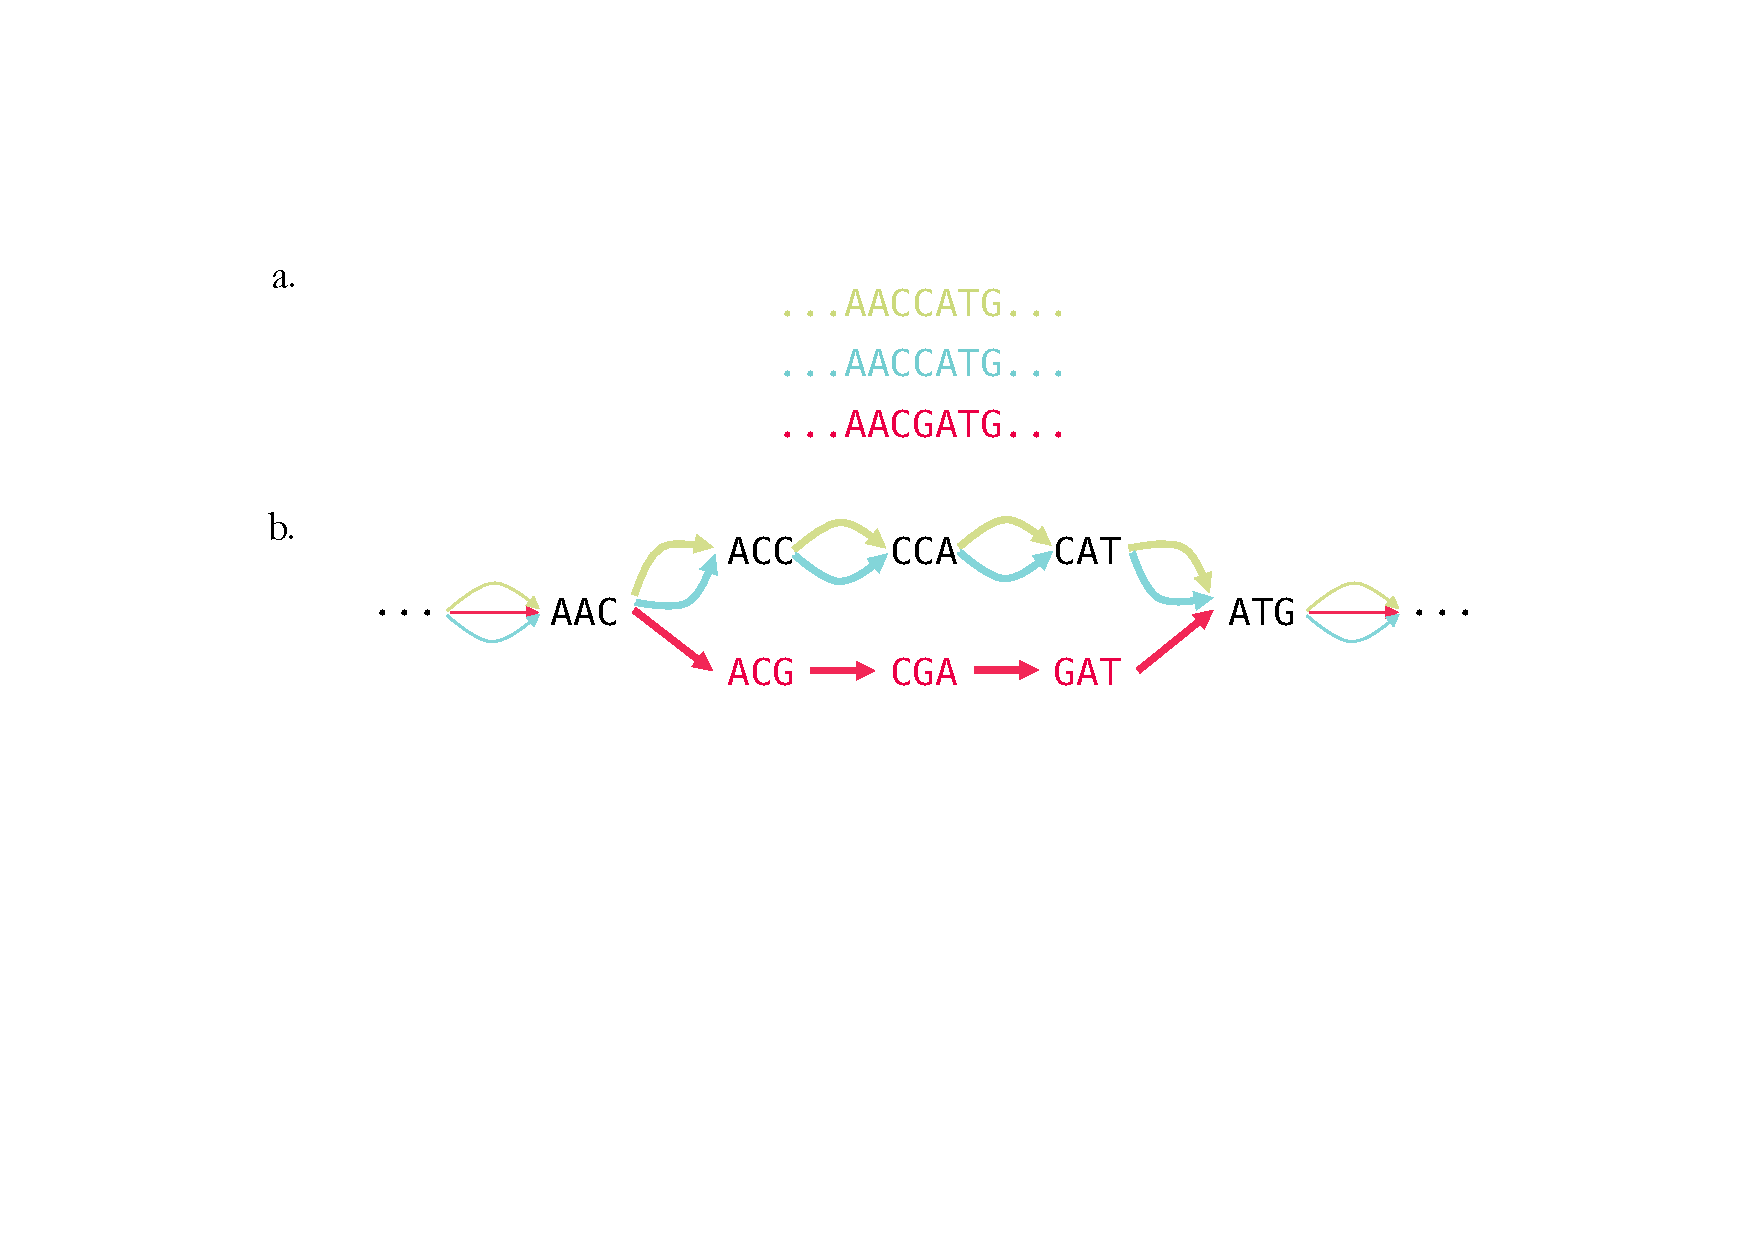
\includegraphics[width=\textwidth]{db_graph_cartoon}
  \caption{a. Haploid sequences from a mother (green), father (blue), and child (red), the last differing from the first two by a single SNP.  b. The resulting multi-color de Bruijn graph for $k=3$. Red vertices denote kmers that are deemed "novel", i.e. present in the child and absent in the parents. Edge colors reflect the samples in which the connected pairs of kmers are found. Edges that are part of the bubble (variant call) are displayed with thicker lines.}
  \label{fig:db_graph_cartoon}
\end{figure}

\begin{figure}[h!]
  \centering
    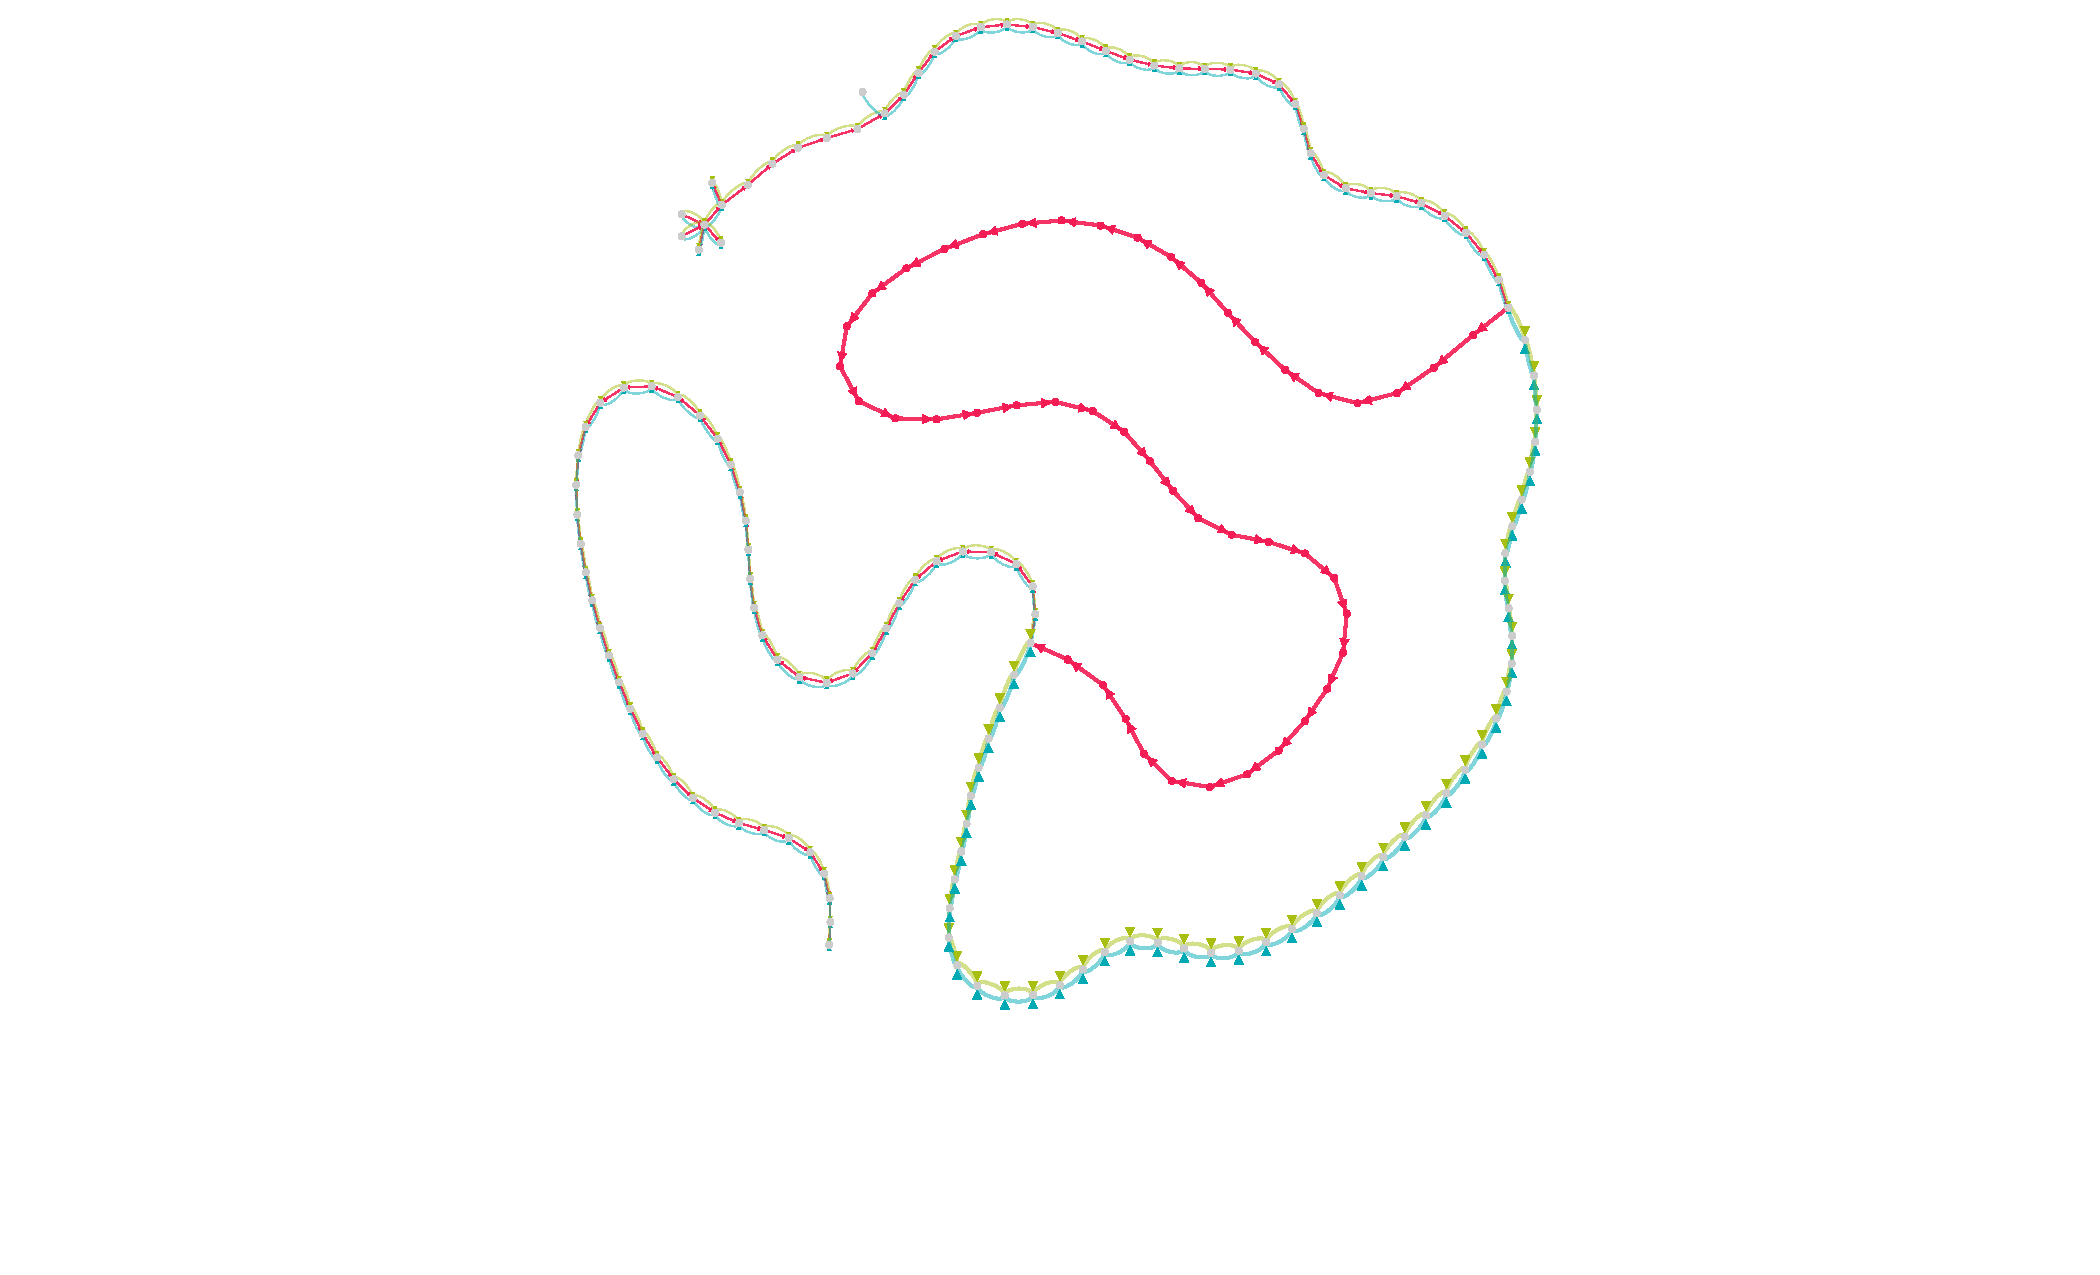
\includegraphics[width=0.5\textwidth]{snp_no_errors}
  \caption{A multi-color de Bruijn graph at $k=47$ for a haploid pedigree spanning a simulated \textit{de novo} SNP.  Vertex labels have been supressed for clarity.  Spatial layout is arbitrary and for display purposes only.}
  \label{fig:snp_no_errors}
\end{figure}

All simple variants will have this basic structure: a bubble in the graph that separates the variant samples from the non-variant samples.  The only major difference is the length of each branch: longer for an insertion in the child, shorter for a deletion (note that for short events, this is generally not apparent from the display, as evidenced by figures \ref{fig:ins_no_errors} and \ref{fig:del_no_errors}).

\begin{figure}[h!]
  \centering
    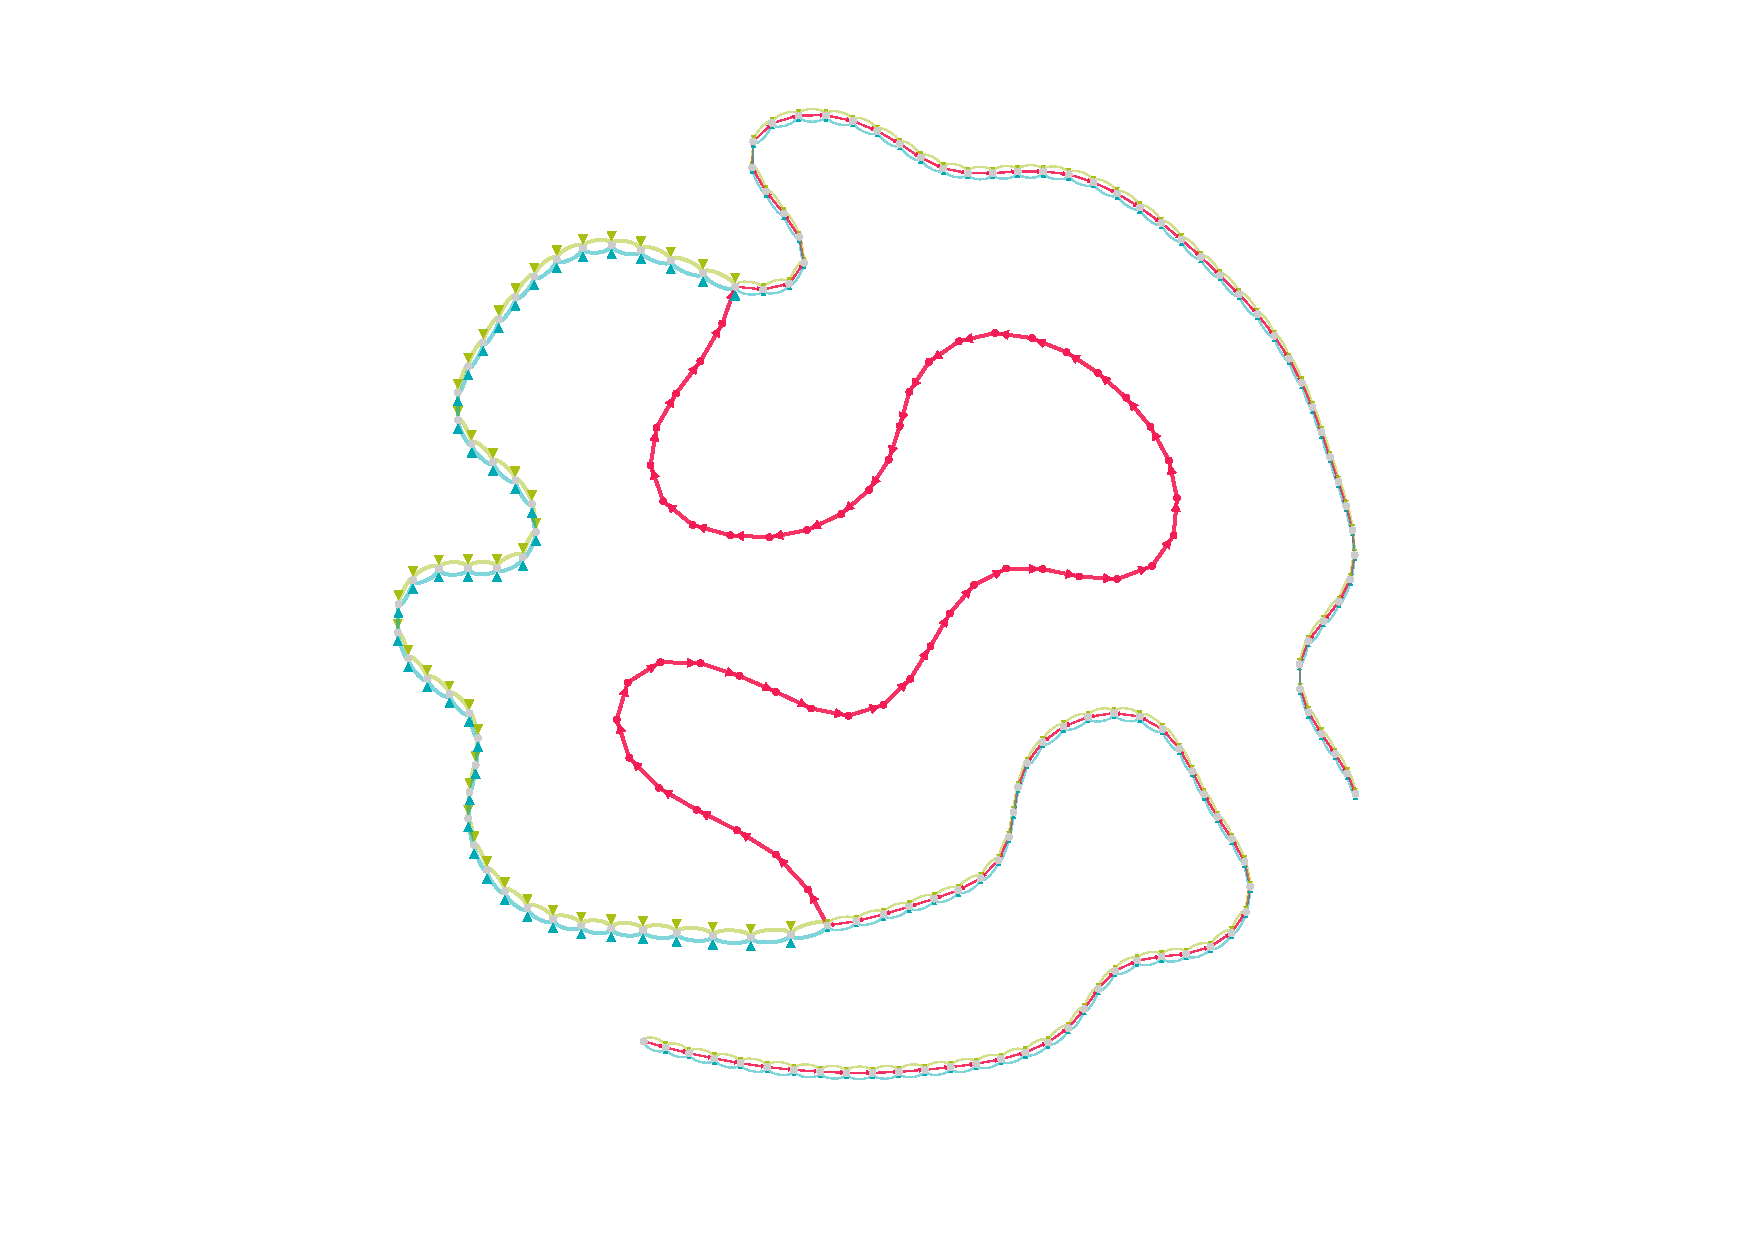
\includegraphics[width=0.5\textwidth]{ins_no_errors}
  \caption{A $5$ bp insertion in the child}
  \label{fig:ins_no_errors}
\end{figure}

\begin{figure}[h!]
  \centering
    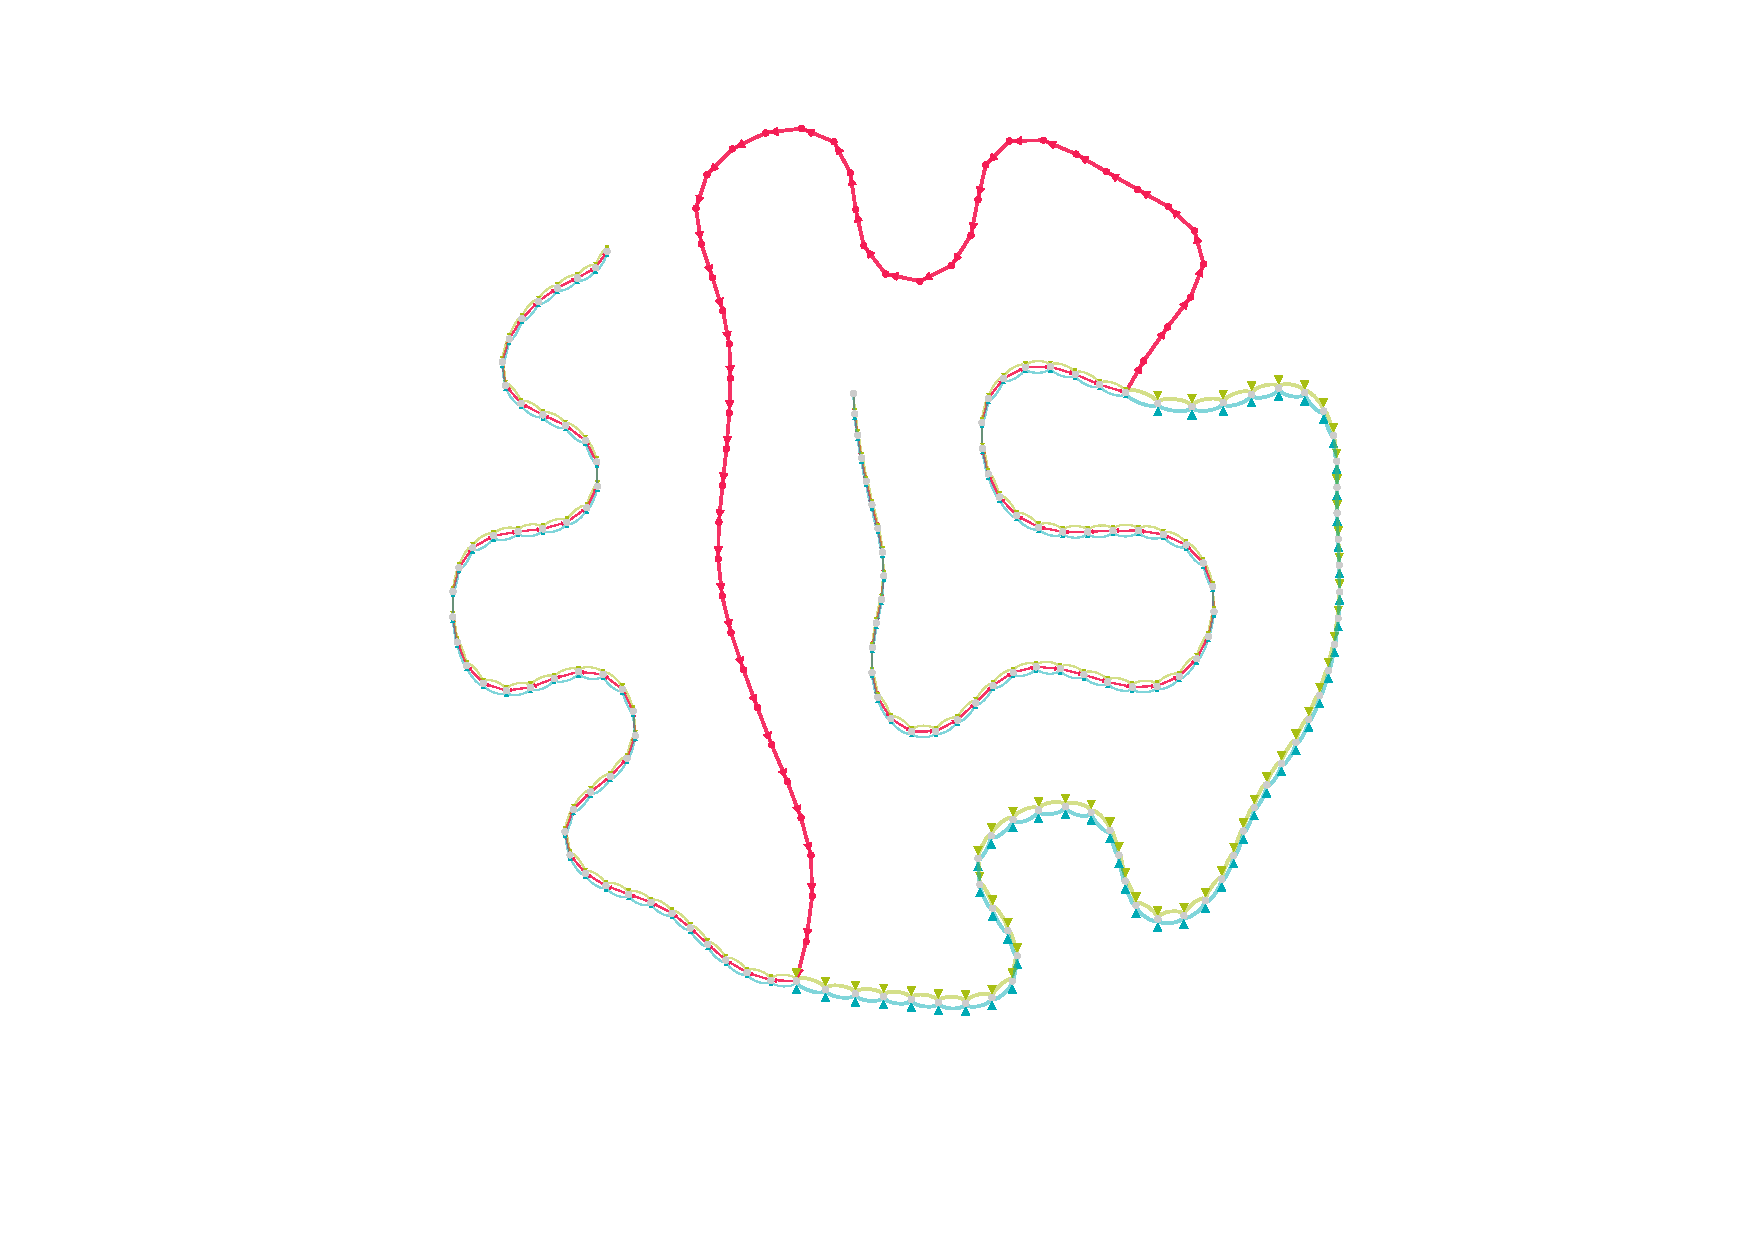
\includegraphics[width=0.5\textwidth]{del_no_errors}
  \caption{A $5$ bp deletion in the child}
  \label{fig:del_no_errors}
\end{figure}

Many variants may occur on the haplotypic background of one parent and not the other.  This is common in regions of the genome that are divergent between the two parents.  Figure \ref{fig:td_haplotypic_background} depicts one such simulated event.  A 41-bp tandem duplication has occurred on the background of the mother (evidenced by the presence of green edges), but not the father (thus the absence of blue edges).  In the flanking tails, edges shared between all three samples are present until a blue edge separates from the graph and connects to different vertices.  While not shown, these branches continue along the genome of the father.

\begin{figure}[h!]
  \centering
    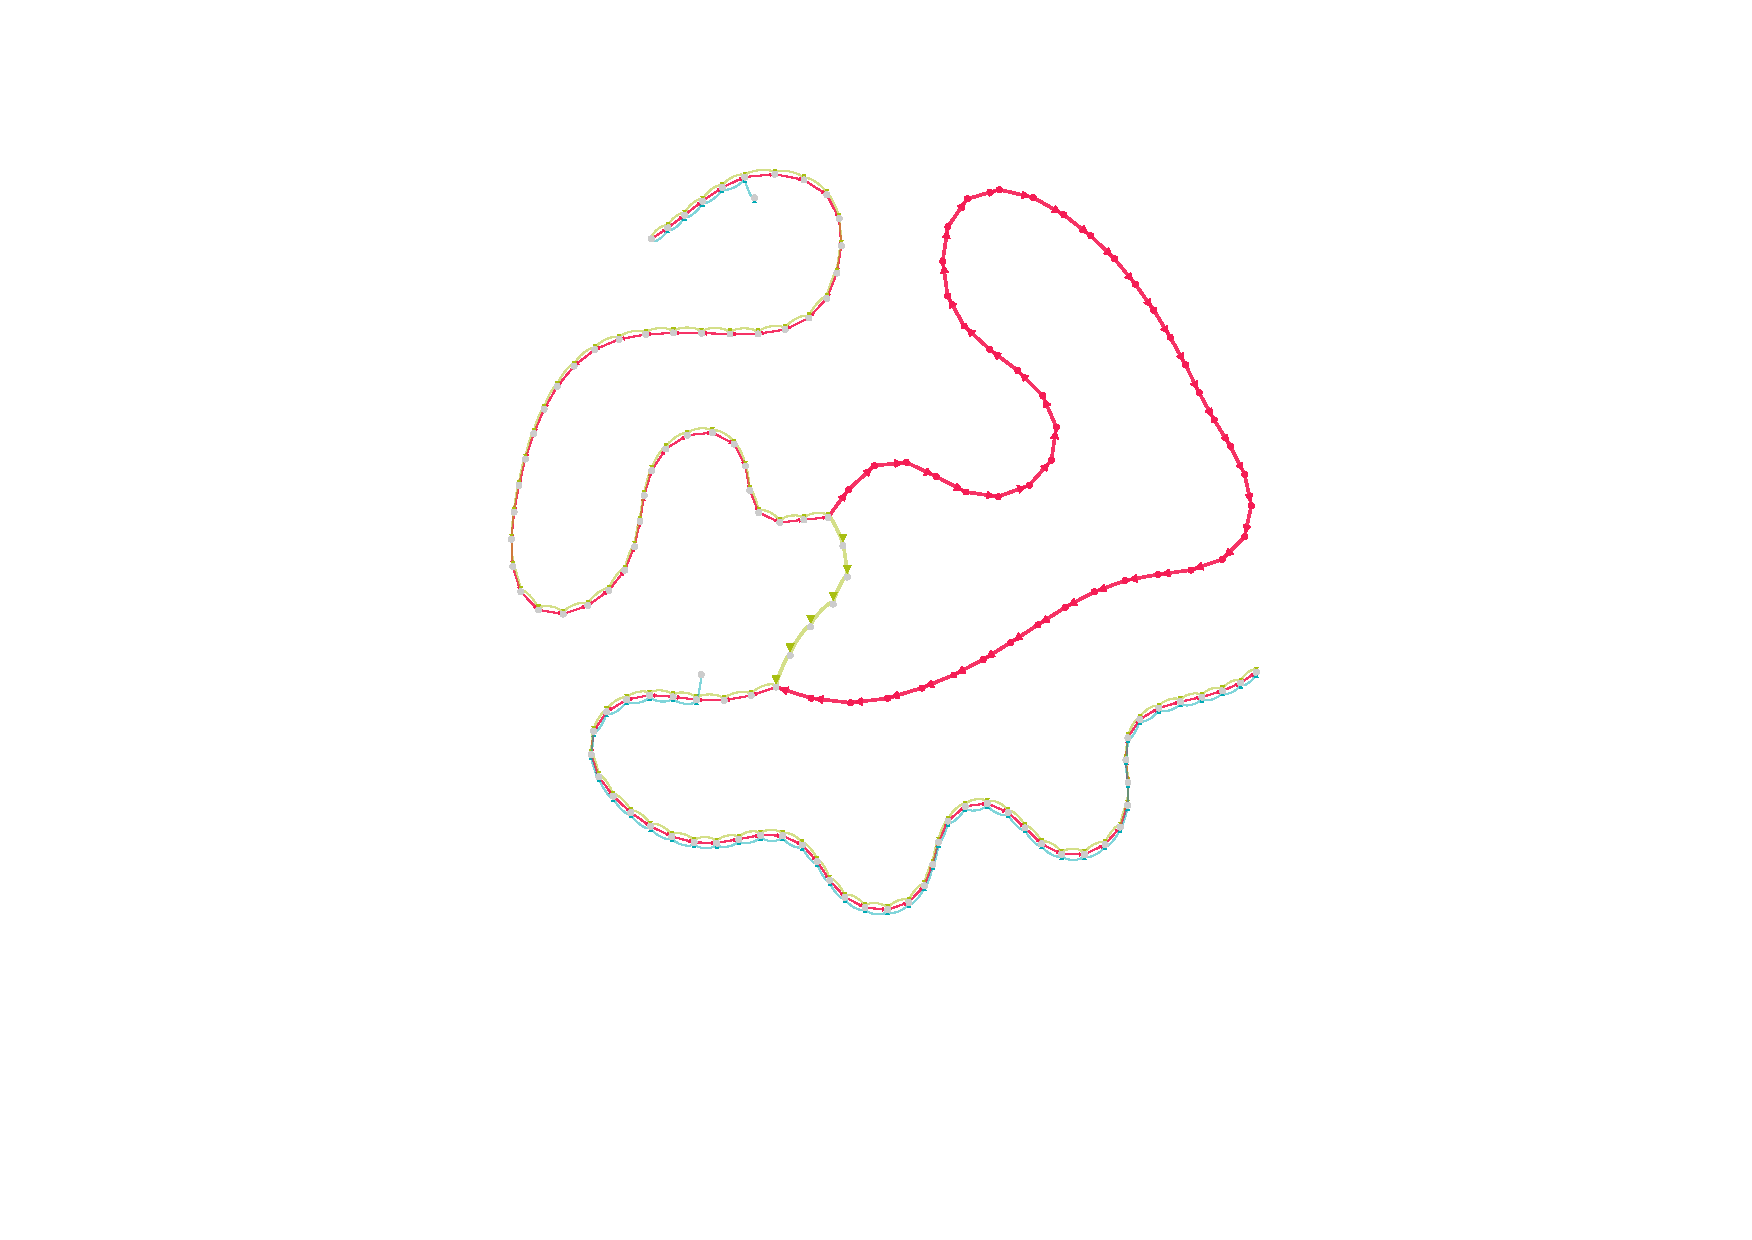
\includegraphics[width=0.5\textwidth]{td_haplotypic_background}
  \caption{A tandem duplication on the haplotypic background of the mother.}
  \label{fig:td_haplotypic_background}
\end{figure}

Finally, it is possible to encounter variants where the path through the graph taken by the child can appear to follow both the variant and non-variant paths, as demonstrated by figure \ref{fig:inv_child_follows_parents}.  Such a scenario may arise by a mutation on a sequence with copy number greater than $1$: both the unaltered and altered sequences would then exist simultaneously in the child's genome.

\begin{figure}[h!]
  \centering
    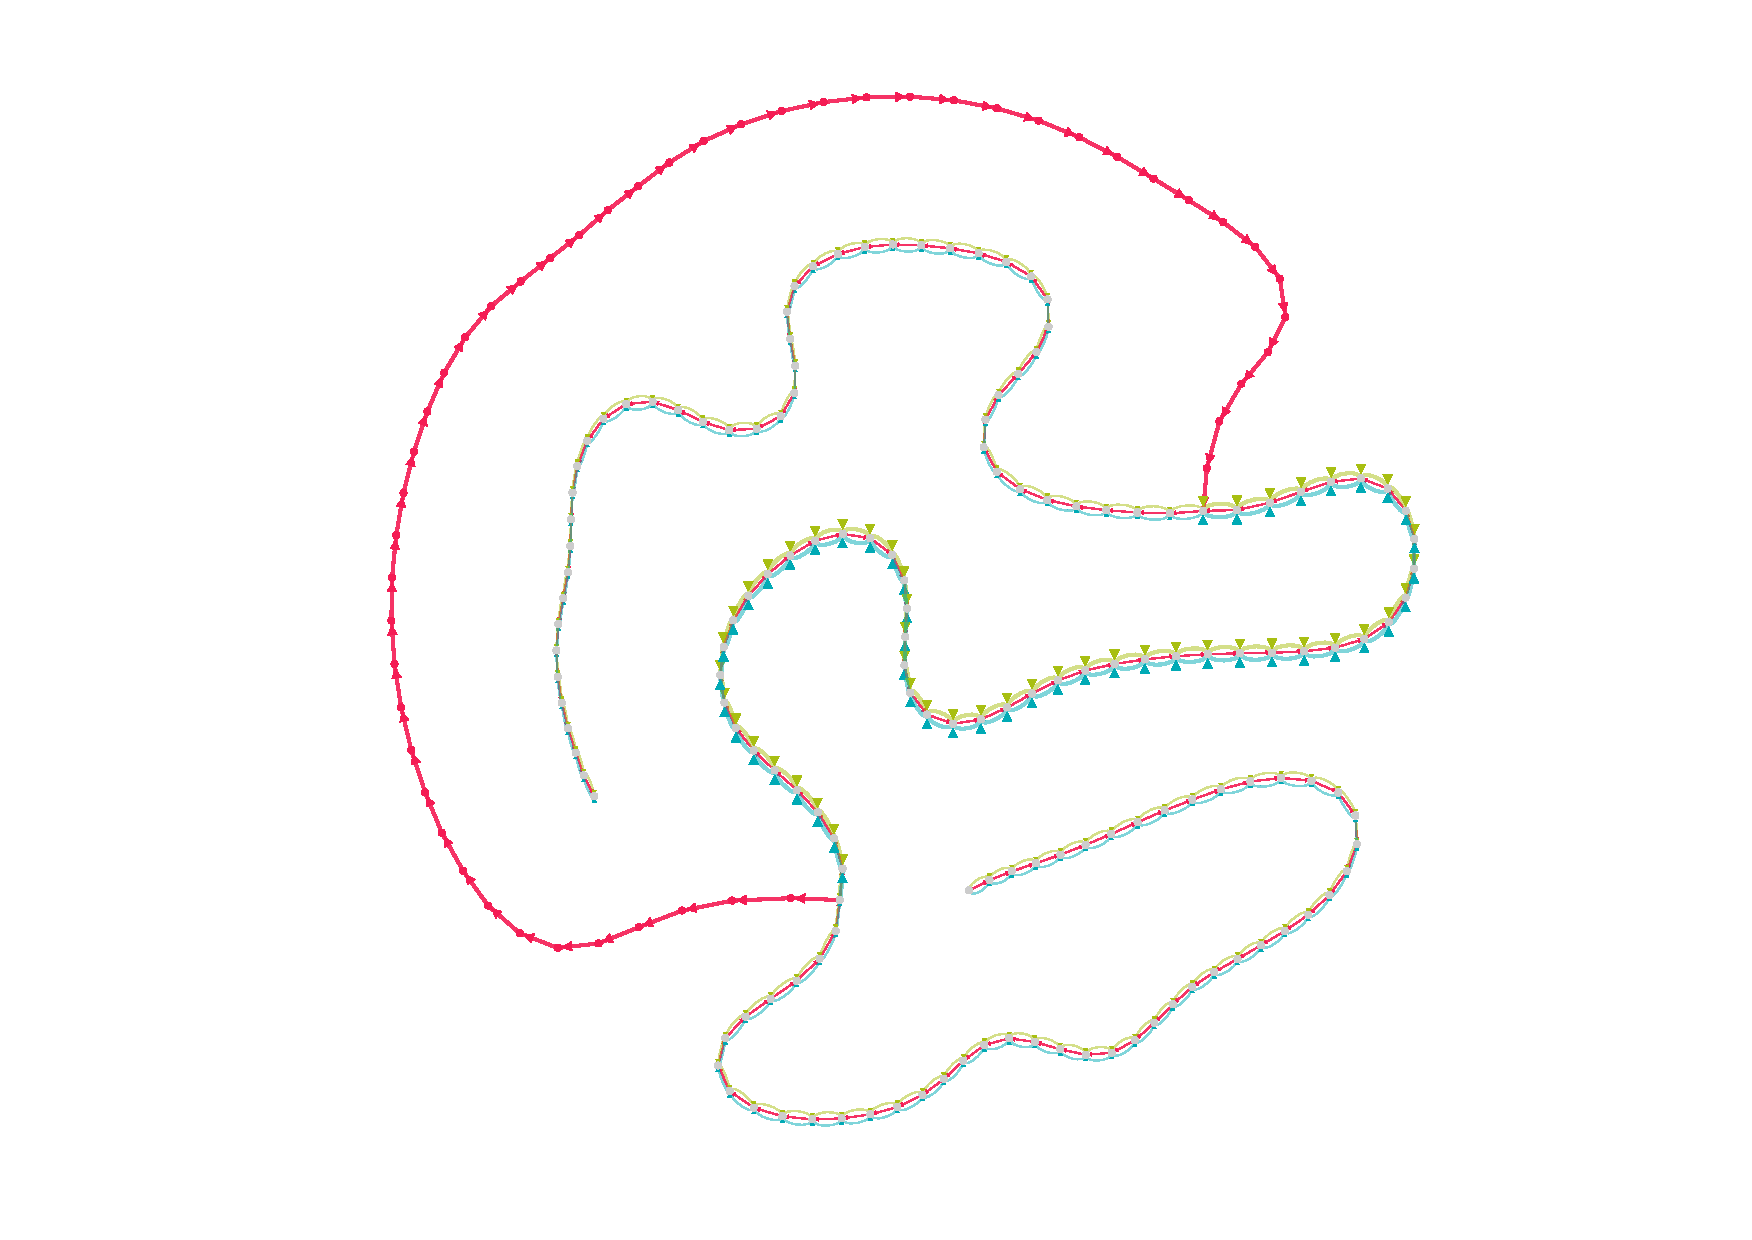
\includegraphics[width=0.5\textwidth]{inv_child_follows_parents}
  \caption{A variant wherein the child's path does not simply diverge from that of the parents, but rather navigates both.}
  \label{fig:inv_child_follows_parents}
\end{figure}

\subsection{Complex variant motifs}

TBW

\subsection{Handling errors in sequencing}

TBW

\section{Calling and classifing \textit{de novo} variants}

Armed with an intuition as to how graphs behave in regions of \textit{de novo} variation, we can now describe the procedure for identifying and classifying a variant.  The overview involves five big steps (and associated substeps):

\begin{enumerate}
\item Identify confident and trusted novel kmers
\item Construct multi-color de Bruijn "trio" graphs (child, mother, father)
\item Load subgraph local to a novel kmer
\item Identify and classify variants in the subgraph
\item Evaluate performance
\end{enumerate}

\subsection{Identify confident and trusted novel kmers}
\subsubsection{Remove low coverage kmers}
\subsubsection{Remove possible contaminants}

\subsection{Construct multi-color de Bruijn "trio" graphs}
\subsubsection{Assemble samples}
\subsubsection{Clean graphs}
\subsubsection{Combine into trio graphs}

\subsection{Load subgraph local to a novel kmer}
\subsubsection{Depth first search}
\subsubsection{Stopping conditions for child}
\subsubsection{Stopping conditions for parents}

\subsection{Identify and classify variants in the subgraph}
\subsubsection{Dijkstra's shortest path algorithm}
\subsubsection{Classify event}
\subsubsection{Mark traversed novel kmers as used}

\subsection{Evaluate performance}
\subsubsection{Generate novel kmer to variant map}
\subsubsection{Load variant containing a novel kmer}
\subsubsection{Compare alleles}

\subsection{Summary}

\section{Results on simulated data}

\begin{table}[]
\centering
\caption{ROC metrics on simulated perfect data}
\label{tbl:roc_perfect}
\begin{tabular}{rlrrrrrrrrrrrrr}
\toprule
sn & sim & fp & fn & tp & tn & rc & sens & spec & prec & npv & fpr & fnr & fdr & acc\\
\midrule
5 & perfect & 1 & 5 & 126 & 22240910 & 9 & 0.9618 & 1 & 0.9921 & 1 & 0 & 0.0382 & 0.0079 & 1\\
3 & perfect & 2 & 3 & 154 & 22200660 & 4 & 0.9809 & 1 & 0.9872 & 1 & 0 & 0.0191 & 0.0128 & 1\\
0 & perfect & 0 & 2 & 106 & 22241343 & 7 & 0.9815 & 1 & 1.0000 & 1 & 0 & 0.0185 & 0.0000 & 1\\
12 & perfect & 0 & 2 & 113 & 22233659 & 3 & 0.9826 & 1 & 1.0000 & 1 & 0 & 0.0174 & 0.0000 & 1\\
13 & perfect & 0 & 2 & 114 & 22217297 & 5 & 0.9828 & 1 & 1.0000 & 1 & 0 & 0.0172 & 0.0000 & 1\\
17 & perfect & 0 & 2 & 117 & 22242890 & 6 & 0.9832 & 1 & 1.0000 & 1 & 0 & 0.0168 & 0.0000 & 1\\
1 & perfect & 1 & 2 & 137 & 22249556 & 8 & 0.9856 & 1 & 0.9928 & 1 & 0 & 0.0144 & 0.0072 & 1\\
14 & perfect & 2 & 2 & 162 & 22196410 & 7 & 0.9878 & 1 & 0.9878 & 1 & 0 & 0.0122 & 0.0122 & 1\\
11 & perfect & 1 & 1 & 114 & 22207761 & 2 & 0.9913 & 1 & 0.9913 & 1 & 0 & 0.0087 & 0.0087 & 1\\
6 & perfect & 1 & 1 & 118 & 22203683 & 2 & 0.9916 & 1 & 0.9916 & 1 & 0 & 0.0084 & 0.0084 & 1\\
8 & perfect & 1 & 1 & 129 & 22229379 & 5 & 0.9923 & 1 & 0.9923 & 1 & 0 & 0.0077 & 0.0077 & 1\\
10 & perfect & 0 & 1 & 130 & 22238480 & 2 & 0.9924 & 1 & 1.0000 & 1 & 0 & 0.0076 & 0.0000 & 1\\
15 & perfect & 1 & 1 & 131 & 22208991 & 10 & 0.9924 & 1 & 0.9924 & 1 & 0 & 0.0076 & 0.0076 & 1\\
16 & perfect & 1 & 1 & 166 & 22213928 & 4 & 0.9940 & 1 & 0.9940 & 1 & 0 & 0.0060 & 0.0060 & 1\\
2 & perfect & 1 & 0 & 105 & 22225262 & 3 & 1.0000 & 1 & 0.9906 & 1 & 0 & 0.0000 & 0.0094 & 1\\
4 & perfect & 2 & 0 & 72 & 22210167 & 2 & 1.0000 & 1 & 0.9730 & 1 & 0 & 0.0000 & 0.0270 & 1\\
7 & perfect & 1 & 0 & 57 & 22225612 & 1 & 1.0000 & 1 & 0.9828 & 1 & 0 & 0.0000 & 0.0172 & 1\\
9 & perfect & 0 & 0 & 107 & 22255460 & 2 & 1.0000 & 1 & 1.0000 & 1 & 0 & 0.0000 & 0.0000 & 1\\
18 & perfect & 2 & 0 & 133 & 22242522 & 0 & 1.0000 & 1 & 0.9852 & 1 & 0 & 0.0000 & 0.0148 & 1\\
19 & perfect & 1 & 0 & 98 & 22236313 & 6 & 1.0000 & 1 & 0.9899 & 1 & 0 & 0.0000 & 0.0101 & 1\\
\bottomrule
\end{tabular}
\end{table}

\begin{table}[]
\centering
\caption{ROC metrics on simulated realistic data}
\label{tbl:roc_realistic}
\begin{tabular}{rlrrrrrrrrrrrrr}
\toprule
sn & sim & fp & fn & tp & tn & rc & sens & spec & prec & npv & fpr & fnr & fdr & acc\\
\midrule
5 & realistic & 4 & 2 & 123 & 77566161 & 7 & 0.9840 & 1 & 0.9685 & 1 & 0 & 0.0160 & 0.0315 & 1\\
0 & realistic & 1 & 1 & 101 & 77516712 & 7 & 0.9902 & 1 & 0.9902 & 1 & 0 & 0.0098 & 0.0098 & 1\\
6 & realistic & 2 & 1 & 107 & 77289511 & 2 & 0.9907 & 1 & 0.9817 & 1 & 0 & 0.0093 & 0.0183 & 1\\
13 & realistic & 0 & 1 & 107 & 77362132 & 3 & 0.9907 & 1 & 1.0000 & 1 & 0 & 0.0093 & 0.0000 & 1\\
17 & realistic & 3 & 1 & 109 & 77390562 & 5 & 0.9909 & 1 & 0.9732 & 1 & 0 & 0.0091 & 0.0268 & 1\\
12 & realistic & 2 & 1 & 111 & 77440516 & 3 & 0.9911 & 1 & 0.9823 & 1 & 0 & 0.0089 & 0.0177 & 1\\
16 & realistic & 1 & 1 & 155 & 77369055 & 5 & 0.9936 & 1 & 0.9936 & 1 & 0 & 0.0064 & 0.0064 & 1\\
2 & realistic & 4 & 0 & 93 & 77425427 & 1 & 1.0000 & 1 & 0.9588 & 1 & 0 & 0.0000 & 0.0412 & 1\\
4 & realistic & 3 & 0 & 65 & 77312705 & 2 & 1.0000 & 1 & 0.9559 & 1 & 0 & 0.0000 & 0.0441 & 1\\
3 & realistic & 6 & 0 & 150 & 77296380 & 1 & 1.0000 & 1 & 0.9615 & 1 & 0 & 0.0000 & 0.0385 & 1\\
1 & realistic & 1 & 0 & 133 & 77509177 & 5 & 1.0000 & 1 & 0.9925 & 1 & 0 & 0.0000 & 0.0075 & 1\\
7 & realistic & 4 & 0 & 56 & 77445270 & 1 & 1.0000 & 1 & 0.9333 & 1 & 0 & 0.0000 & 0.0667 & 1\\
8 & realistic & 6 & 0 & 126 & 77469034 & 3 & 1.0000 & 1 & 0.9545 & 1 & 0 & 0.0000 & 0.0455 & 1\\
9 & realistic & 2 & 0 & 95 & 77503142 & 2 & 1.0000 & 1 & 0.9794 & 1 & 0 & 0.0000 & 0.0206 & 1\\
10 & realistic & 1 & 0 & 124 & 77398963 & 2 & 1.0000 & 1 & 0.9920 & 1 & 0 & 0.0000 & 0.0080 & 1\\
11 & realistic & 2 & 0 & 108 & 77422535 & 2 & 1.0000 & 1 & 0.9818 & 1 & 0 & 0.0000 & 0.0182 & 1\\
14 & realistic & 6 & 0 & 150 & 77355056 & 7 & 1.0000 & 1 & 0.9615 & 1 & 0 & 0.0000 & 0.0385 & 1\\
15 & realistic & 1 & 0 & 125 & 77435743 & 9 & 1.0000 & 1 & 0.9921 & 1 & 0 & 0.0000 & 0.0079 & 1\\
18 & realistic & 4 & 0 & 123 & 77355144 & 3 & 1.0000 & 1 & 0.9685 & 1 & 0 & 0.0000 & 0.0315 & 1\\
19 & realistic & 2 & 0 & 95 & 77480228 & 6 & 1.0000 & 1 & 0.9794 & 1 & 0 & 0.0000 & 0.0206 & 1\\
\bottomrule
\end{tabular}
\end{table}

\begin{figure}[h!]
  \centering
    \includegraphics[width=\textwidth]{{conf.perfect.hm-1}.pdf}
  \caption{Confusion matrix for observed events (below) versus expected events (right), in simulated perfect data.}
  \label{fig:conf_perfect_hm}
\end{figure}

\begin{figure}[h!]
  \centering
    \includegraphics[width=\textwidth]{{conf.realistic.hm-1}.pdf}
  \caption{Confusion matrix for observed events (below) versus expected events (right), in simulated realistic data.}
  \label{fig:conf_realistic_hm}
\end{figure}

\begin{figure}[h!]
  \centering
    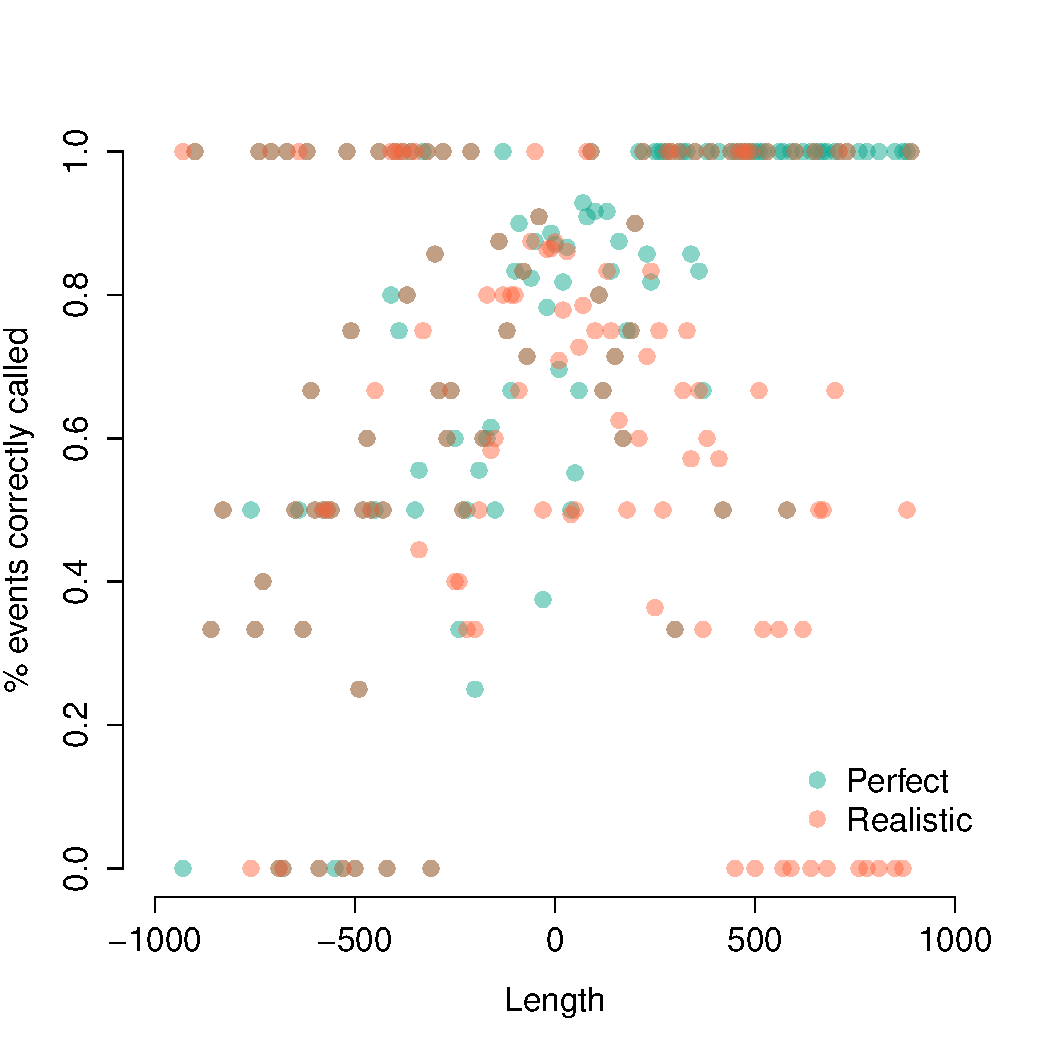
\includegraphics[width=\textwidth]{lengthHit-1}
  \caption{Event recovery as a function of event length}
  \label{fig:lengthHit}
\end{figure}
